\def\year{2021}\relax
%File: formatting-instructions-latex-2021.tex
%release 2021.1
\documentclass[letterpaper]{article} % DO NOT CHANGE THIS
\usepackage{aaai21}  % DO NOT CHANGE THIS
\usepackage{times}  % DO NOT CHANGE THIS
\usepackage{helvet} % DO NOT CHANGE THIS
\usepackage{courier}  % DO NOT CHANGE THIS
\usepackage[hyphens]{url}  % DO NOT CHANGE THIS
\usepackage{graphicx} % DO NOT CHANGE THIS
\urlstyle{rm} % DO NOT CHANGE THIS
\def\UrlFont{\rm}  % DO NOT CHANGE THIS
\usepackage{natbib}  % DO NOT CHANGE THIS AND DO NOT ADD ANY OPTIONS TO IT
\usepackage{caption} % DO NOT CHANGE THIS AND DO NOT ADD ANY OPTIONS TO IT
\frenchspacing  % DO NOT CHANGE THIS
\setlength{\pdfpagewidth}{8.5in}  % DO NOT CHANGE THIS
\setlength{\pdfpageheight}{11in}  % DO NOT CHANGE THIS



% New Packages Added Here:
\usepackage{xcolor}
\usepackage{amsmath,amssymb}
\usepackage{calrsfs}
\DeclareMathAlphabet{\pazocal}{OMS}{zplm}{m}{n}

\usepackage{multirow}
\usepackage{makeidx}
\usepackage{graphicx}
\usepackage{amsmath,amssymb} % define this before the line numbering.
\usepackage{color}
\renewcommand{\ttdefault}{pcr}
\usepackage{graphicx}
\usepackage{float}
\usepackage{subcaption}
\usepackage{color}
\newcommand{\MK}[1]{{\textcolor{red}{\it[Margret: #1]}}\xspace}
% Definition of \GCPRreviewversion which
% defines the use of line numbers etc.
\usepackage{graphicx}
\usepackage{booktabs}

\def\imagetop#1{\vtop{\null\hbox{#1}}}

%\nocopyright
%PDF Info Is REQUIRED.
% For /Author, add all authors within the parentheses, separated by commas. No accents or commands.
% For /Title, add Title in Mixed Case. No accents or commands. Retain the parentheses.
\pdfinfo{
/Title (AAAI Press Formatting Instructions for Authors Using LaTeX -- A Guide)
/Author (AAAI Press Staff, Pater Patel Schneider, Sunil Issar, J. Scott Penberthy, George Ferguson, Hans Guesgen, Francisco Cruz, Marc Pujol-Gonzalez)
/TemplateVersion (2021.1)
} %Leave this
% /Title ()
% Put your actual complete title (no codes, scripts, shortcuts, or LaTeX commands) within the parentheses in mixed case
% Leave the space between \Title and the beginning parenthesis alone
% /Author ()
% Put your actual complete list of authors (no codes, scripts, shortcuts, or LaTeX commands) within the parentheses in mixed case.
% Each author should be only by a comma. If the name contains accents, remove them. If there are any LaTeX commands,
% remove them.

% DISALLOWED PACKAGES
% \usepackage{authblk} -- This package is specifically forbidden
% \usepackage{balance} -- This package is specifically forbidden
% \usepackage{color (if used in text)
% \usepackage{CJK} -- This package is specifically forbidden
% \usepackage{float} -- This package is specifically forbidden
% \usepackage{flushend} -- This package is specifically forbidden
% \usepackage{fontenc} -- This package is specifically forbidden
% \usepackage{fullpage} -- This package is specifically forbidden
% \usepackage{geometry} -- This package is specifically forbidden
% \usepackage{grffile} -- This package is specifically forbidden
% \usepackage{hyperref} -- This package is specifically forbidden
% \usepackage{navigator} -- This package is specifically forbidden
% (or any other package that embeds links such as navigator or hyperref)
% \indentfirst} -- This package is specifically forbidden
% \layout} -- This package is specifically forbidden
% \multicol} -- This package is specifically forbidden
% \nameref} -- This package is specifically forbidden
% \usepackage{savetrees} -- This package is specifically forbidden
% \usepackage{setspace} -- This package is specifically forbidden
% \usepackage{stfloats} -- This package is specifically forbidden
% \usepackage{tabu} -- This package is specifically forbidden
% \usepackage{titlesec} -- This package is specifically forbidden
% \usepackage{tocbibind} -- This package is specifically forbidden
% \usepackage{ulem} -- This package is specifically forbidden
% \usepackage{wrapfig} -- This package is specifically forbidden
% DISALLOWED COMMANDS
% \nocopyright -- Your paper will not be published if you use this command
% \addtolength -- This command may not be used
% \balance -- This command may not be used
% \baselinestretch -- Your paper will not be published if you use this command
% \clearpage -- No page breaks of any kind may be used for the final version of your paper
% \columnsep -- This command may not be used
% \newpage -- No page breaks of any kind may be used for the final version of your paper
% \pagebreak -- No page breaks of any kind may be used for the final version of your paperr
% \pagestyle -- This command may not be used
% \tiny -- This is not an acceptable font size.
% \vspace{- -- No negative value may be used in proximity of a caption, figure, table, section, subsection, subsubsection, or reference
% \vskip{- -- No negative value may be used to alter spacing above or below a caption, figure, table, section, subsection, subsubsection, or reference

\setcounter{secnumdepth}{0} %May be changed to 1 or 2 if section numbers are desired.

% The file aaai21.sty is the style file for AAAI Press
% proceedings, working notes, and technical reports.
%

% Title

% Your title must be in mixed case, not sentence case.
% That means all verbs (including short verbs like be, is, using,and go),
% nouns, adverbs, adjectives should be capitalized, including both words in hyphenated terms, while
% articles, conjunctions, and prepositions are lower case unless they
% directly follow a colon or long dash

%\title{Uncertainty and Sparsity Trade-off in the Minimum Cost Lifted Multicut Formulation}
%\title{Uncertainties in Graph Decomposition: %\\
%A Study on Minimum Cost (Lifted) Multicuts}
\title{Spectral Distribution aware Image Generation\\
Supplementary Material}
\author{

    %Authors
    Paper ID: 1900
    % All authors must be in the same font size and format.
    %%Written by AAAI Press Staff\textsuperscript{\rm 1}\thanks{With help from the AAAI Publications Committee.}\\
    %%AAAI Style Contributions by Pater Patel Schneider,
    %%Sunil Issar,  \\
    %%J. Scott Penberthy,
    %%George Ferguson,
    %%Hans Guesgen,
    %%Francisco Cruz,
    %%Marc Pujol-Gonzalez
}
\begin{document}
%
%\title{Contribution Title\thanks{Supported by organization x.}}
%
%\titlerunning{Abbreviated paper title}
% If the paper title is too long for the running head, you can set
% an abbreviated paper title here
%
%\author{First Author\inst{1}\orcidID{0000-1111-2222-3333} \and
%Second Author\inst{2,3}\orcidID{1111-2222-3333-4444} \and
%Third Author\inst{3}\orcidID{2222--3333-4444-5555}}
%
%\authorrunning{F. Author et al.}
% First names are abbreviated in the running head.
% If there are more than two authors, 'et al.' is used.
%
%\institute{Princeton University, Princeton NJ 08544, USA \and
%Springer Heidelberg, Tiergartenstr. 17, 69121 Heidelberg, Germany
%\email{lncs@springer.com}\\
%\url{http://www.springer.com/gp/computer-science/lncs} \and
%ABC Institute, Rupert-Karls-University Heidelberg, Heidelberg, Germany\\
%\email{\{abc,lncs\}@uni-heidelberg.de}}
%
\maketitle              % typeset the header of the contribution
%



\begin{figure}
\centering
\begin{tabular}{@{}c@{}c@{}c@{}}
     \imagetop{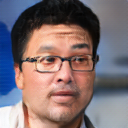
\includegraphics[width=0.32\linewidth]{img/generated_samples/DCGAN128/0294.png}} &
   \imagetop{ 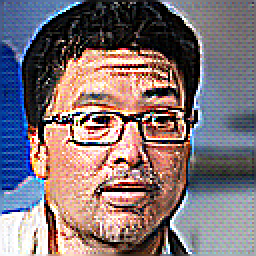
\includegraphics[width=0.32\linewidth]{img/generated_samples/0294_2.png} }&
     \imagetop{   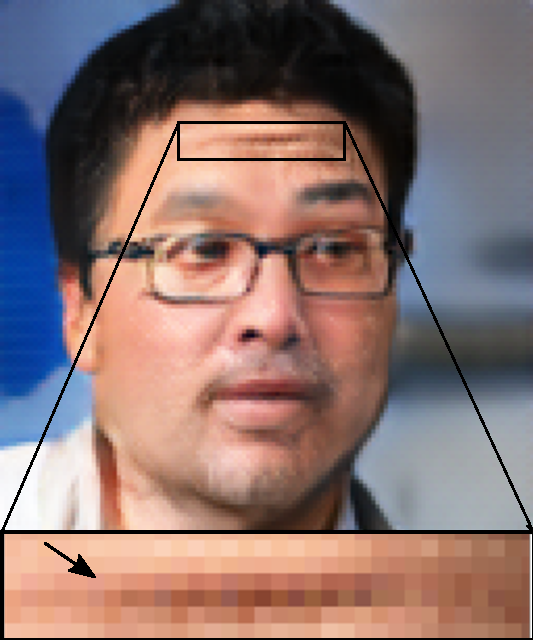
\includegraphics[width=0.32\linewidth]{img/generated_samples/zoom_artifacts.pdf}} \\
        (a) DCGAN&(b) sharpened&(c) zoomed in

\end{tabular}

\caption{Sample from DCGAN, $128^2$. Peaks in the high frequencies which we measure in the power spectrum correspond to grid artifacts in the images. After applying an image sharpening operation, they become obvious (b) but at a close look, they can also be perceived in the original generated images (c). }
\label{fig:sharpened}
\end{figure}
\section{High Frequency Artifacts}
In the proposed paper, we show that frequency artifacts in generated images can be significantly removed be using a simple spectral discriminator. Here, we want to emphasize again why a peak in the high frequency regime of the generated images' power spectra are undesired. We provide an example in Figure \ref{fig:sharpened}, showing a face in front of what appears to be a mostly homogeneous background. Yet after applying a sharpening operation (Fig.\ref{fig:sharpened}(b)) , grid artifacts become obvious even in these supposedly flat regions. At a close look, they can also be seen in the plain images without sharpening (Fig.\ref{fig:sharpened}(c)).

\section{Training Stability of Durall et al. (CVPR 2020)}
Next, we compare the training stability of the proposed method with the one from \cite{margret2020upconvolution}. We show in Figure \ref{fig:y equals x} the FID over 500 training epochs for five runs of the model from \cite{margret2020upconvolution}. Two out of five of these runs collapsed before reaching epoch 200. Below in Figure \ref{fig:three sin x}, we show the same experiment for the proposed model, where not only the training runs stably but also the resulting FID is lower.

\begin{figure}
    \centering
    \begin{subfigure}[b]{\linewidth}
        \centering
        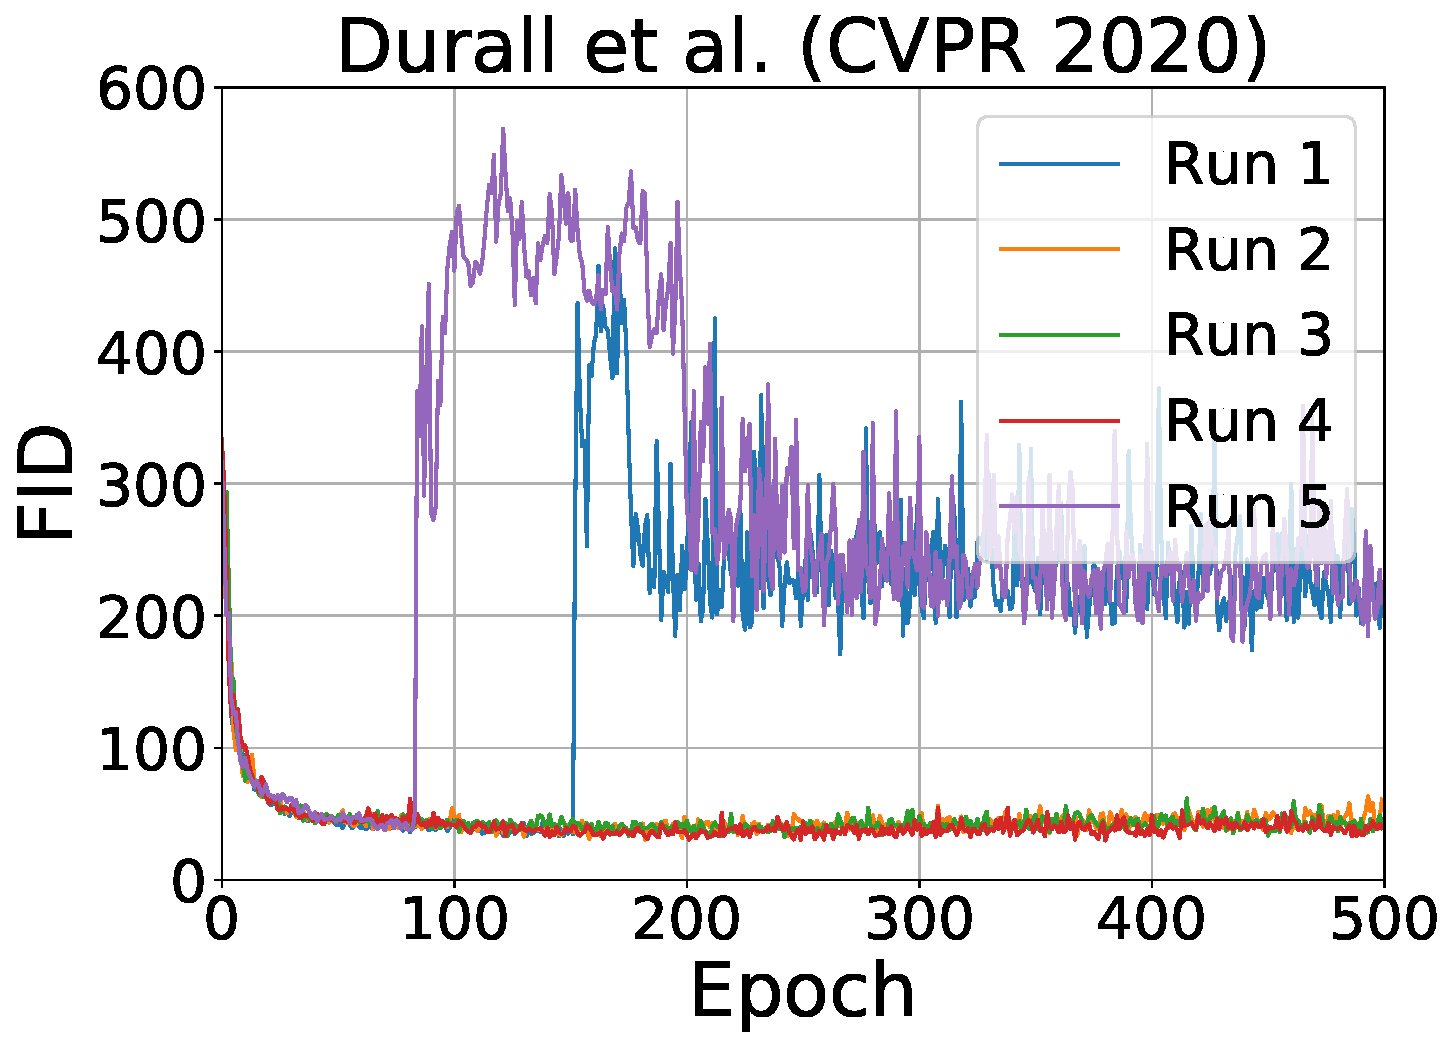
\includegraphics[width=\linewidth]{img/stability_baseline.pdf}
        \caption{$2$ out of $5$ runs are unstable using the implementation provided by Durall et al.}
        \label{fig:y equals x}
    \end{subfigure}
    \hfill
    \begin{subfigure}[b]{\linewidth}
        \centering
        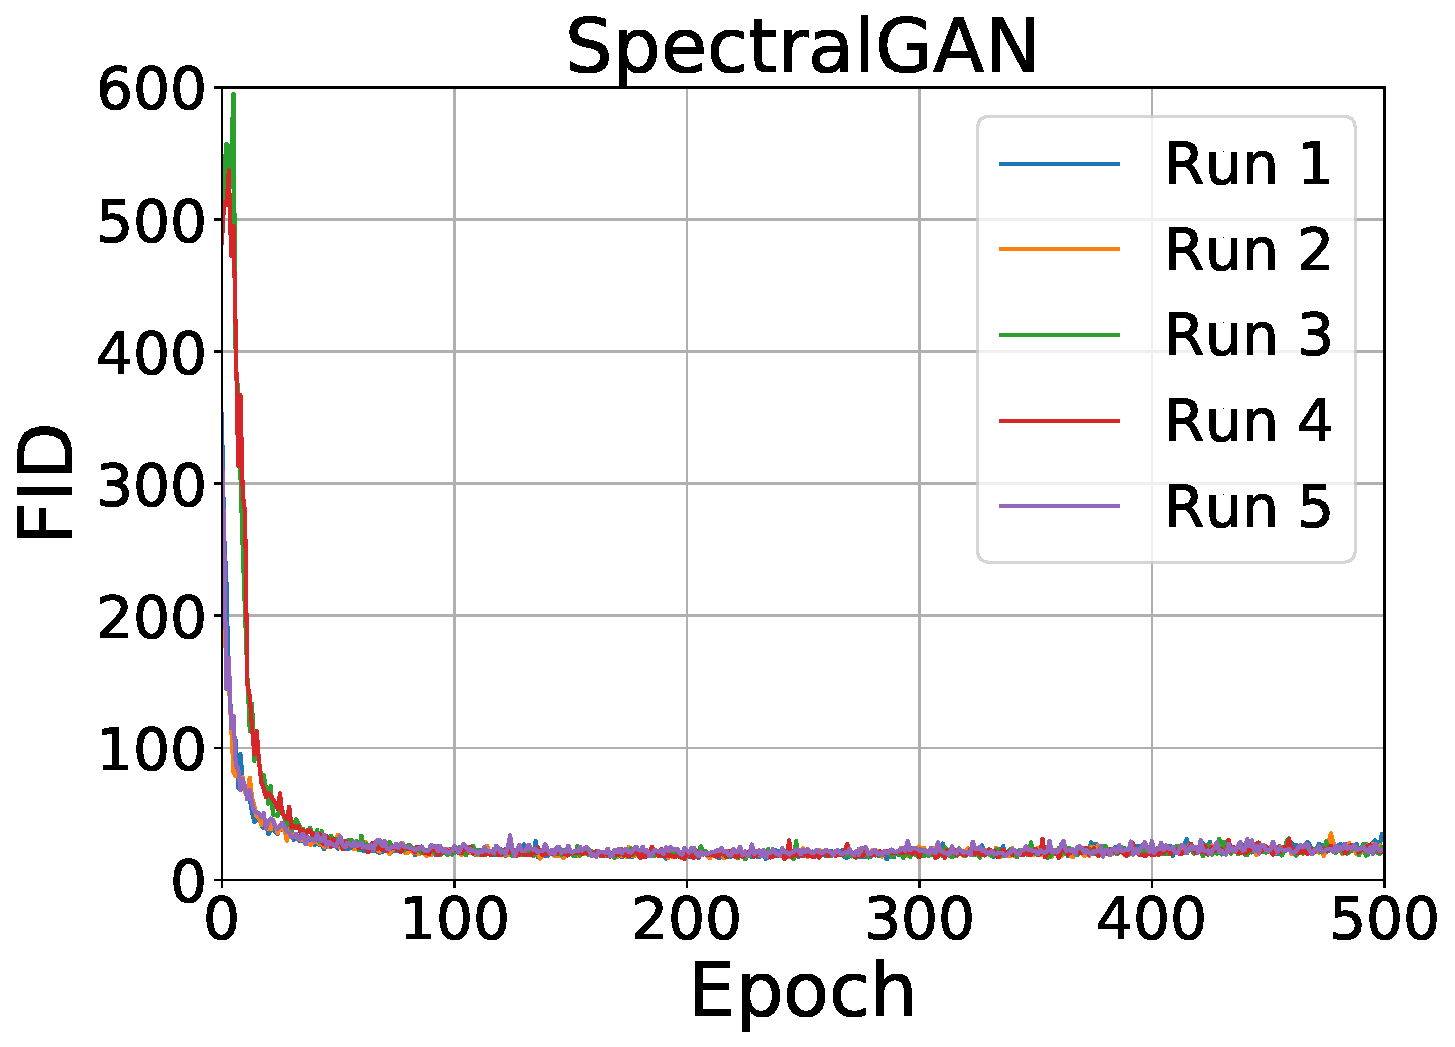
\includegraphics[width=\linewidth]{img/stability_spectral.pdf}
        \caption{All of our $5$ runs are stable.}
        \label{fig:three sin x}
    \end{subfigure}
    \caption{Comparison of the training stability of Durall et al. and our proposed method. The training was run for $500$ epochs on $64^2$ resolutions using the DCGAN loss.}
    \label{fig:three graphs}
\end{figure}
\section{Additional Evaluation of Generated Power Spectra}
Figure \ref{fig:spec_baseline} shows the mean absolute differences of the 2D power spectra of real and generated images as in Fig. 5 of the main paper. Here, we compare the spectra resulting from DCGAN (Figure \ref{fig:spec_baseline} (a)), from DCGAn with the spectral regularization from \citet{margret2020upconvolution} (Figure \ref{fig:spec_baseline} (b)) and our proposed model (Figure \ref{fig:spec_baseline} (c)). With the proposed model, the mean differences are significantly smaller even in the 2D power spectral, although the discriminator only operates on 1D projections of the spectra. The 2D spectra of the reference method \cite{margret2020upconvolution} still exhibit strong deviations.  
\begin{figure}
\scriptsize
\begin{tabular}{@{\hspace{0cm}}c@{\hspace{0cm}}c@{}c@{}c@{}c@{}c@{}c@{}c@{}}
\imagetop{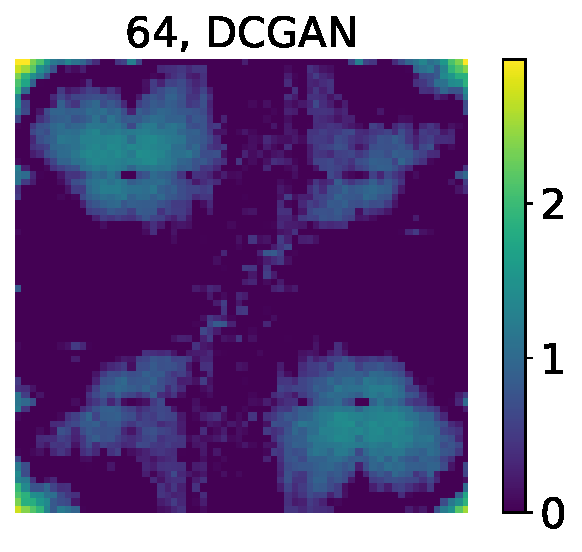
\includegraphics[width=0.33\linewidth]{img/img_2/Spectrum_64_DCGAN.pdf}}&
\imagetop{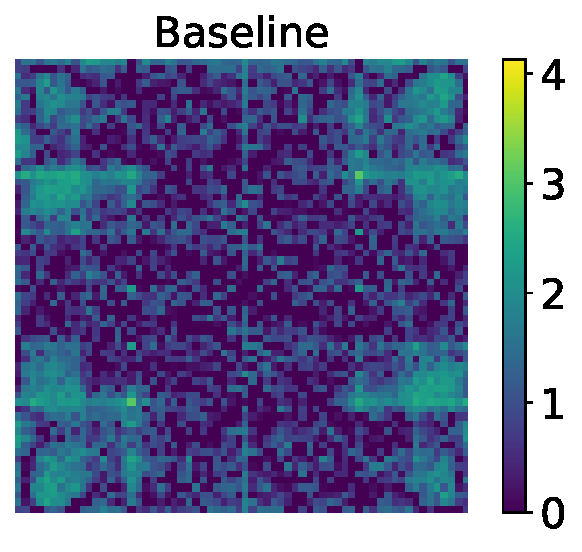
\includegraphics[width=0.33\linewidth]{img/img_2/Spectrum_Baseline.pdf}}&
\imagetop{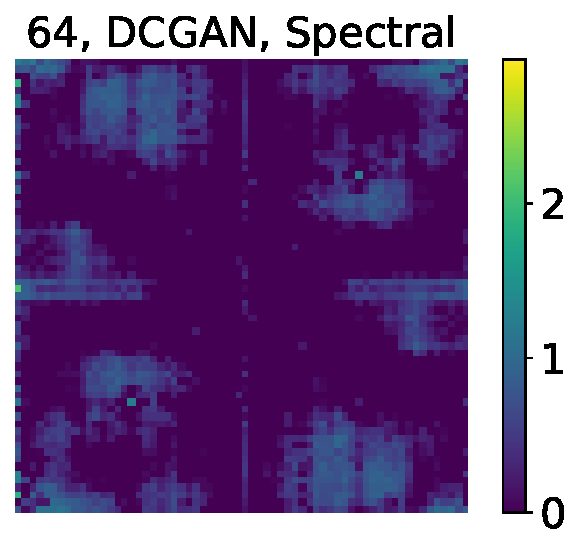
\includegraphics[width=0.33\linewidth]{img/img_2/Spectrum_64_DCGAN_Spectral.pdf}}\\
(a) DCGAN $64\times64$& (b) Durall et al., CVPR'20& (c) DCGAN Spectral
\end{tabular}
\caption{Average magnitude differences of the 2D FFT between real and generated images. We compare (a) DCGAN without additional loss or regularization, (b) DCGAN with the regularization proposed in \cite{margret2020upconvolution} and (c) the proposed model with spectral discriminator.}
\label{fig:spec_baseline}
\end{figure}
In Figure \ref{fig:cloaking2} we report the mean and standard deviation of the spectral profiles (azimuthal integrals) of the proposed model for higher resolution images. As shown in the maim paper for images of resolution $64\times 64$, the distributions fit almost perfectly when our proposed discriminator is use. Figure \ref{fig:cloaking2} shows the corresponding plots for resolutions $128\times 128$ and $256\times256$. In both cases, the 1D projections of the power spectra are very similarly distributed when our model is used while they show obvious differences otherwise.
\begin{figure}[!ht]%[h!]
\scriptsize
\begin{tabular}{@{\hspace{0cm}}c@{\hspace{0cm}}c@{\hspace{0cm}}}
   % \begin{subfigure}[t]{.3\textwidth}
    %    \centering
    \iffalse
        \includegraphics[width=0.49\linewidth]{img/img_2/64, DCGAN.pdf}&
        \includegraphics[width=0.49\linewidth]{img/img_2/64, DCGAN, Spectral.pdf}\\
        $64\times 64 $ DCGAN& DCGAN Spectral\\
        \includegraphics[width=0.49\linewidth]{img/img_2/64, LSGAN.pdf}&
        \includegraphics[width=0.49\linewidth]{img/img_2/64, LSGAN, Spectral.pdf}\\
        $64\times 64 $ LSGAN& LSGAN Spectral\\
                \includegraphics[width=0.49\linewidth]{img/img_2/64, WGAN.pdf}&
        \includegraphics[width=0.49\linewidth]{img/img_2/64, WGAN, Spectral.pdf}\\
       $64\times 64 $  WGAN& WGAN Spectral\\
        \includegraphics[width=0.49\linewidth]{img/img_2/64, WGAN-GP.pdf}&
        \includegraphics[width=0.49\linewidth]{img/img_2/64, WGAN-GP, Spectral.pdf}\\
        $64\times 64 $ WGAN-GP& WGAN-GP Spectral\\
        \fi
        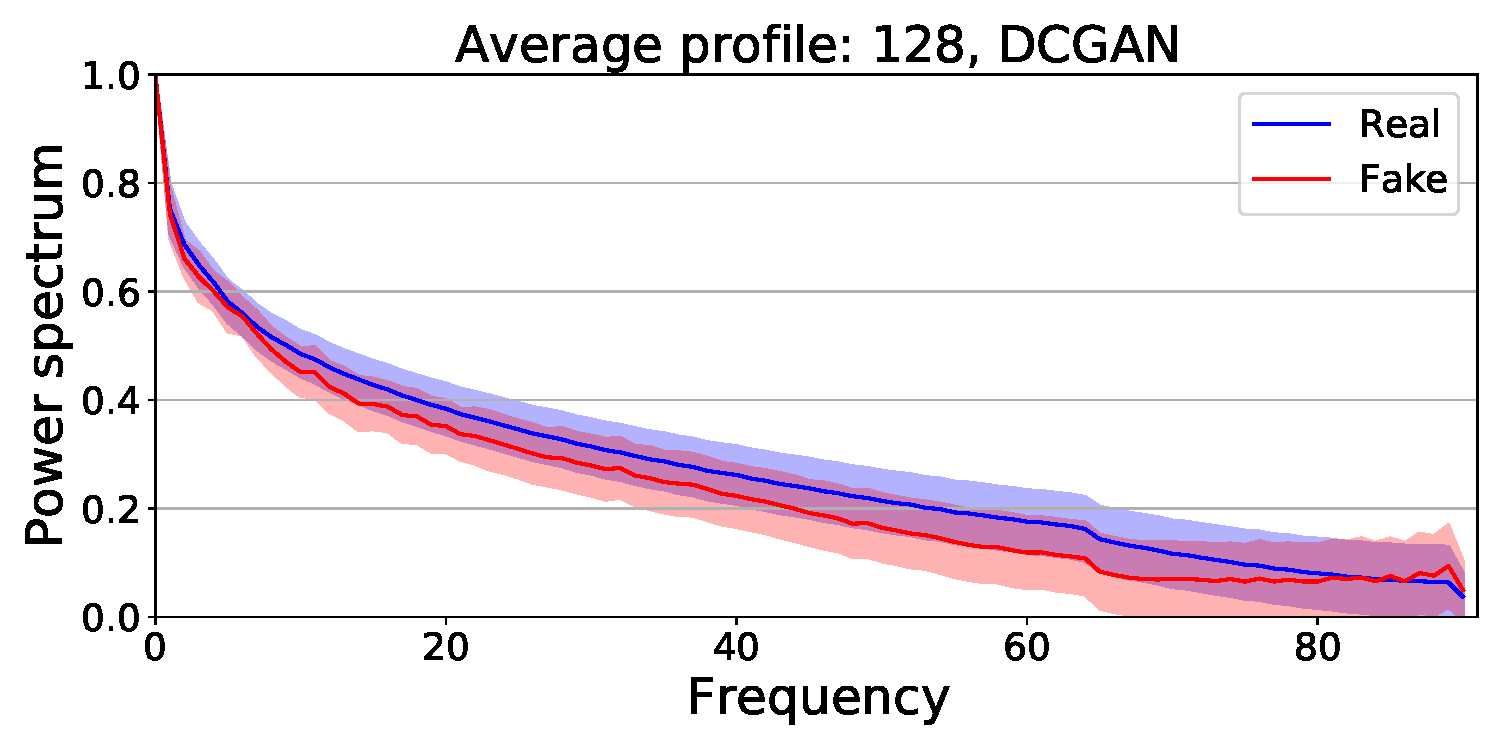
\includegraphics[width=0.49\linewidth]{img/img_2/128_DCGAN.pdf}&
        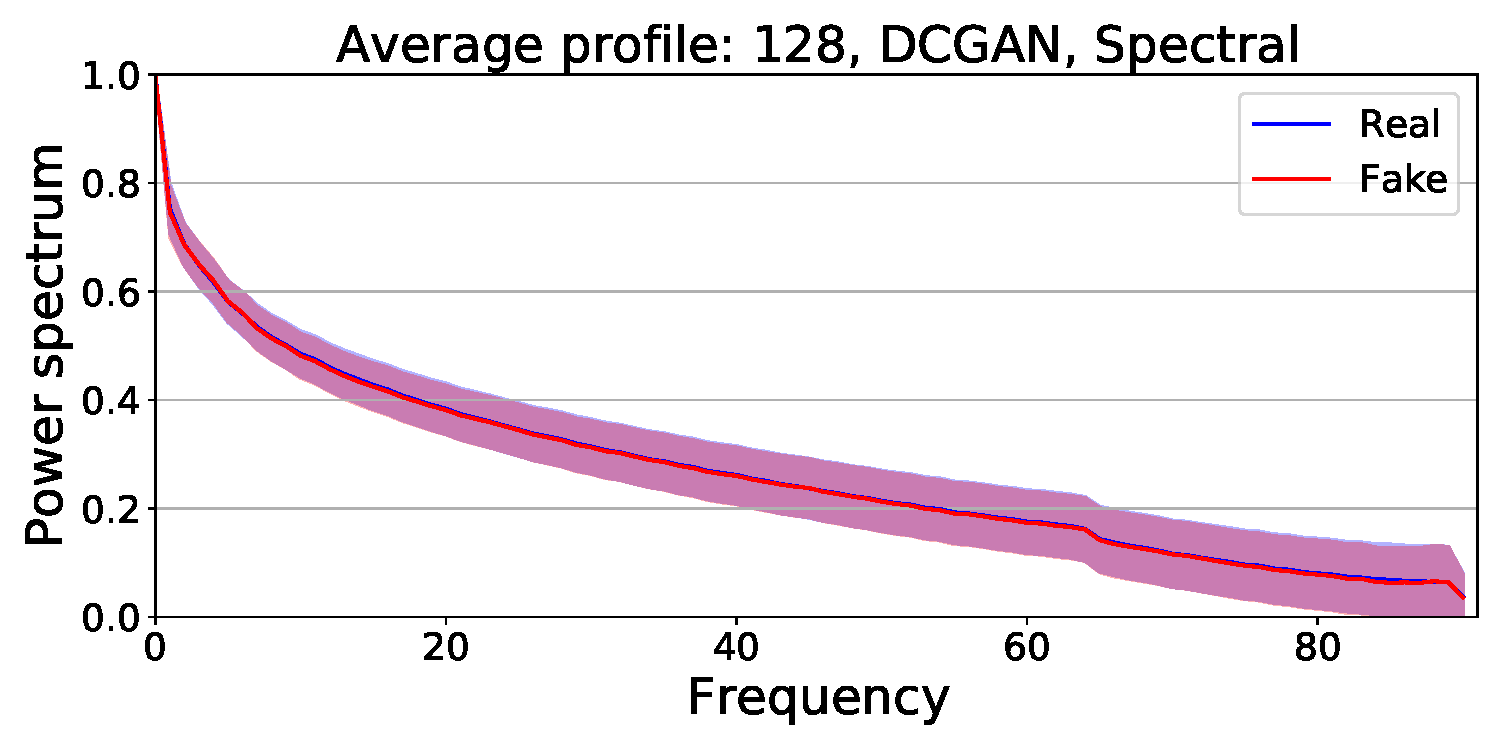
\includegraphics[width=0.49\linewidth]{img/img_2/128_DCGAN_Spectral.pdf}\\
        $128\times 128 $ DCGAN& DCGAN Spectral\\
        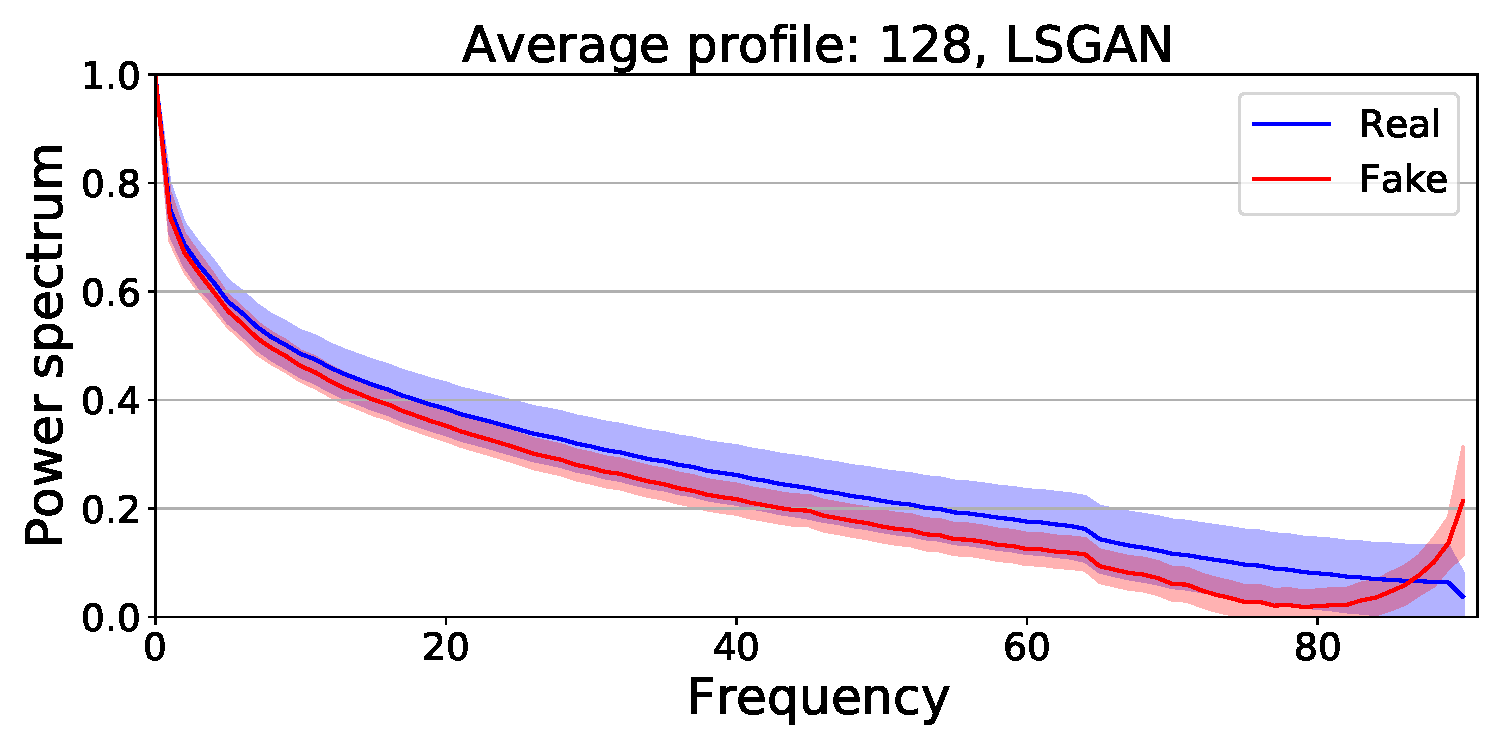
\includegraphics[width=0.49\linewidth]{img/img_2/128_LSGAN.pdf}&
        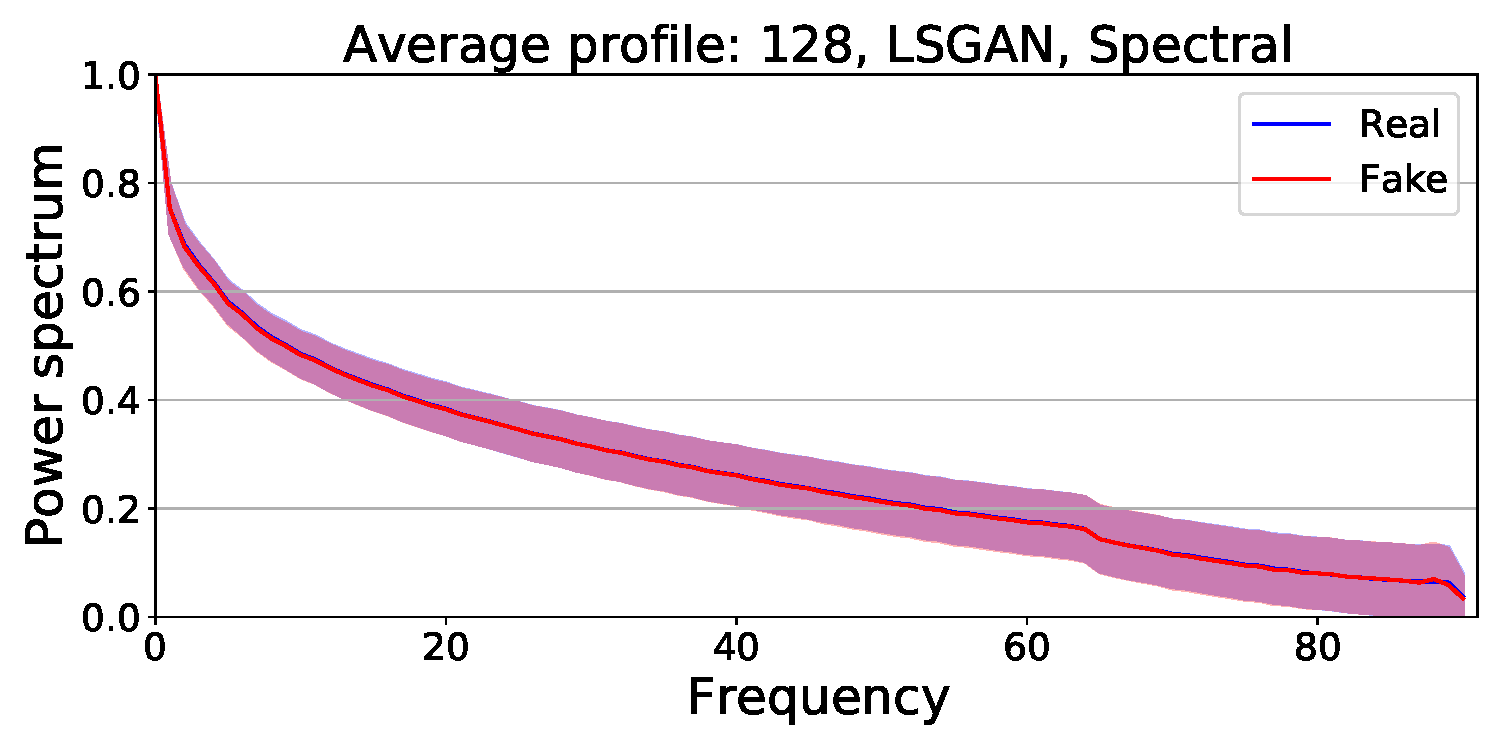
\includegraphics[width=0.49\linewidth]{img/img_2/128_LSGAN_Spectral.pdf}\\
        $128\times 128 $ LSGAN& LSGAN Spectral\\
                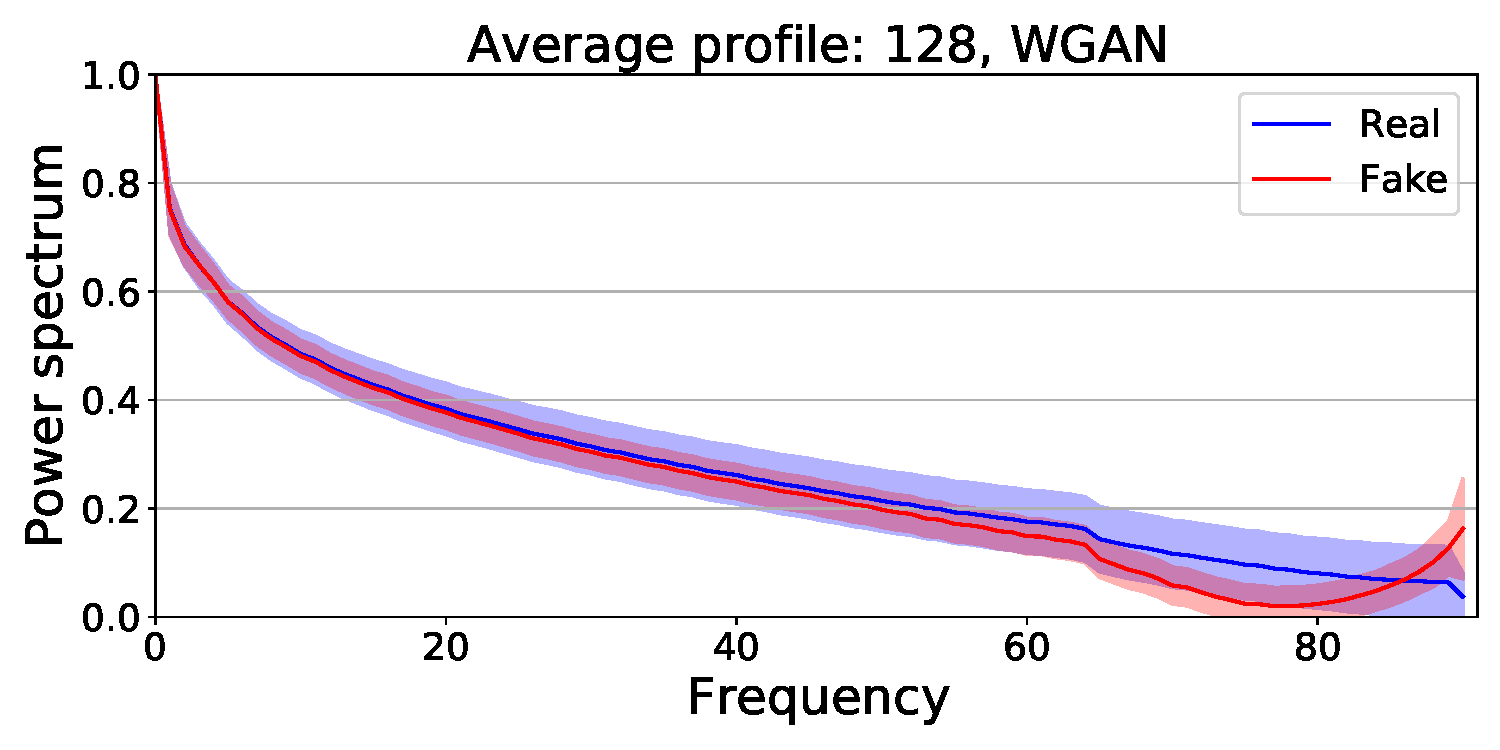
\includegraphics[width=0.49\linewidth]{img/img_2/128_WGAN.pdf}&
        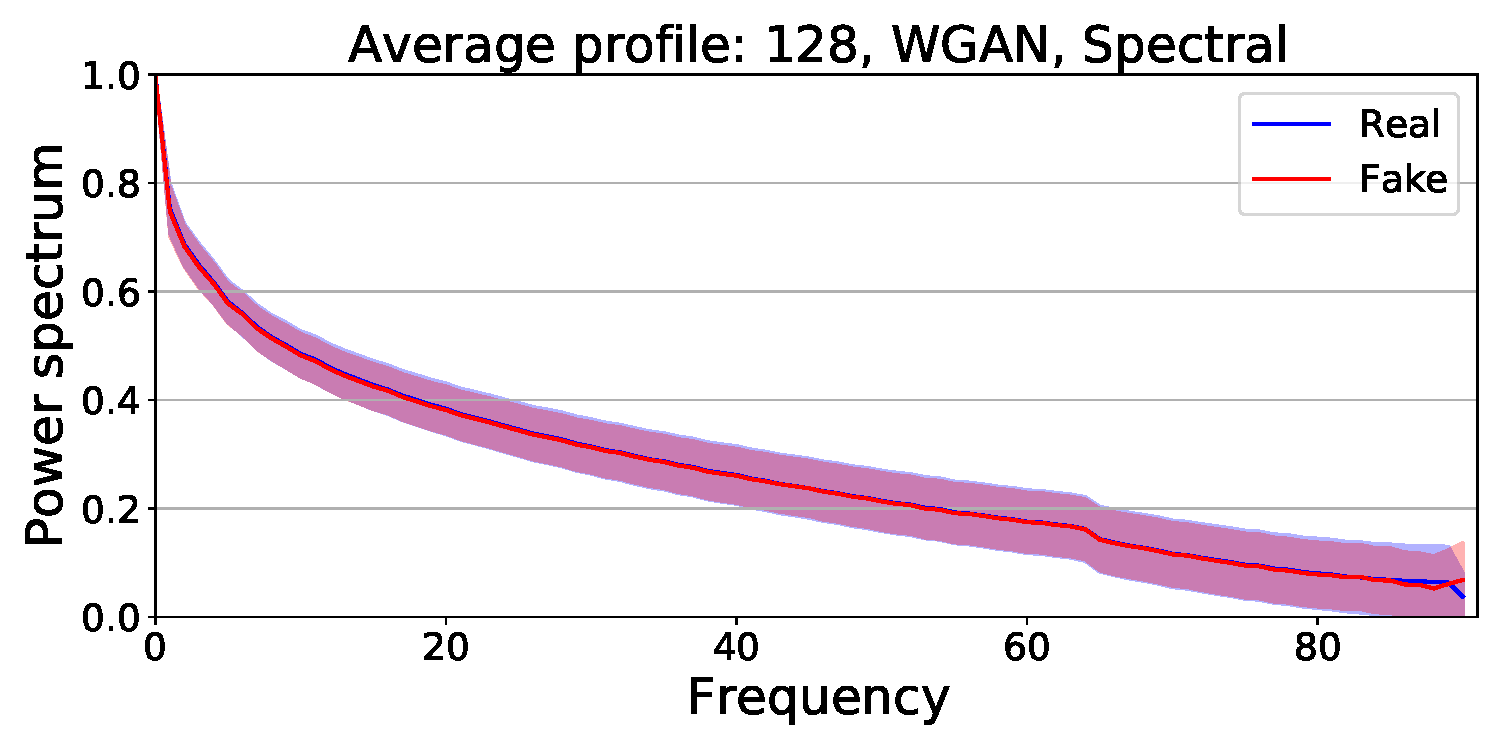
\includegraphics[width=0.49\linewidth]{img/img_2/128_WGAN_Spectral.pdf}\\
        $128\times 128 $ WGAN& WGAN Spectral\\
        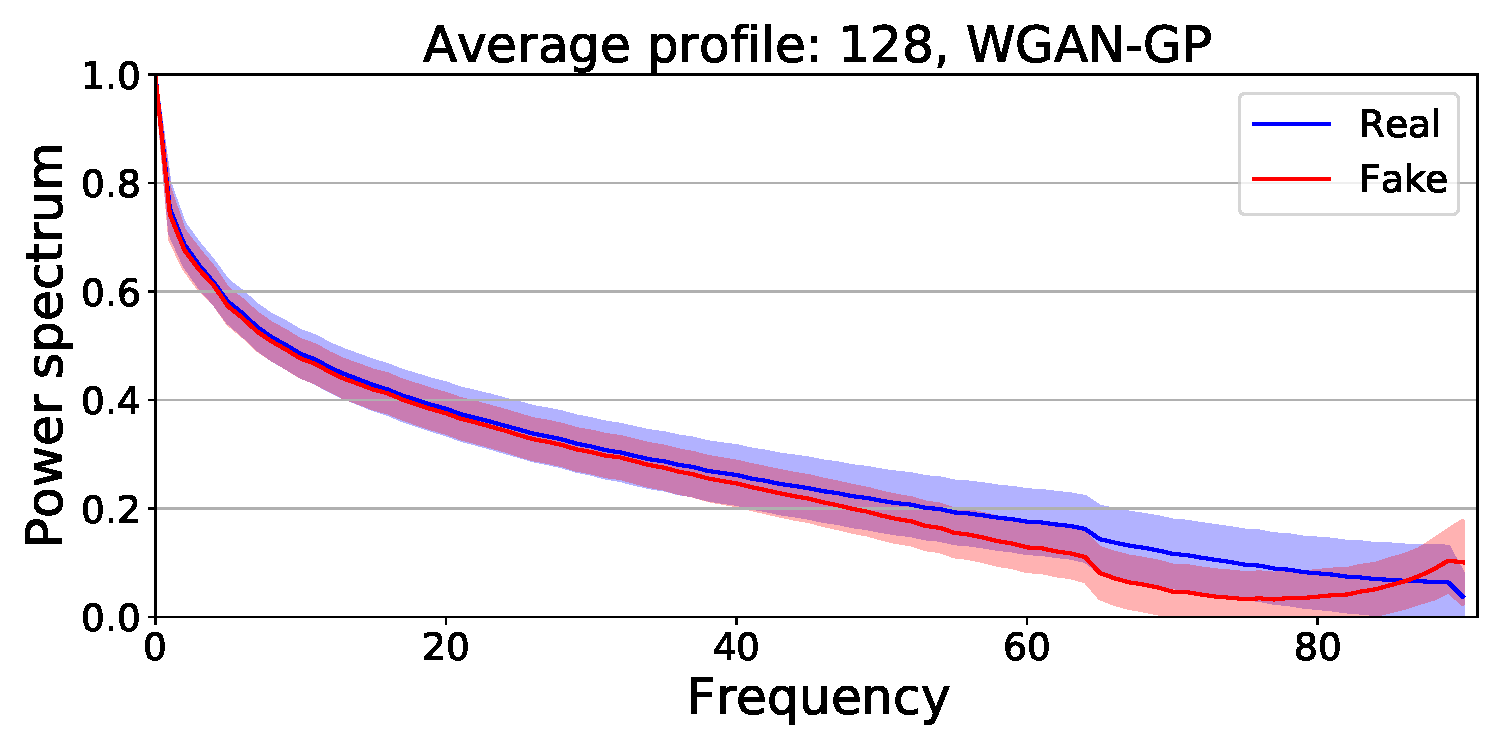
\includegraphics[width=0.49\linewidth]{img/img_2/128_WGAN-GP.pdf}&
        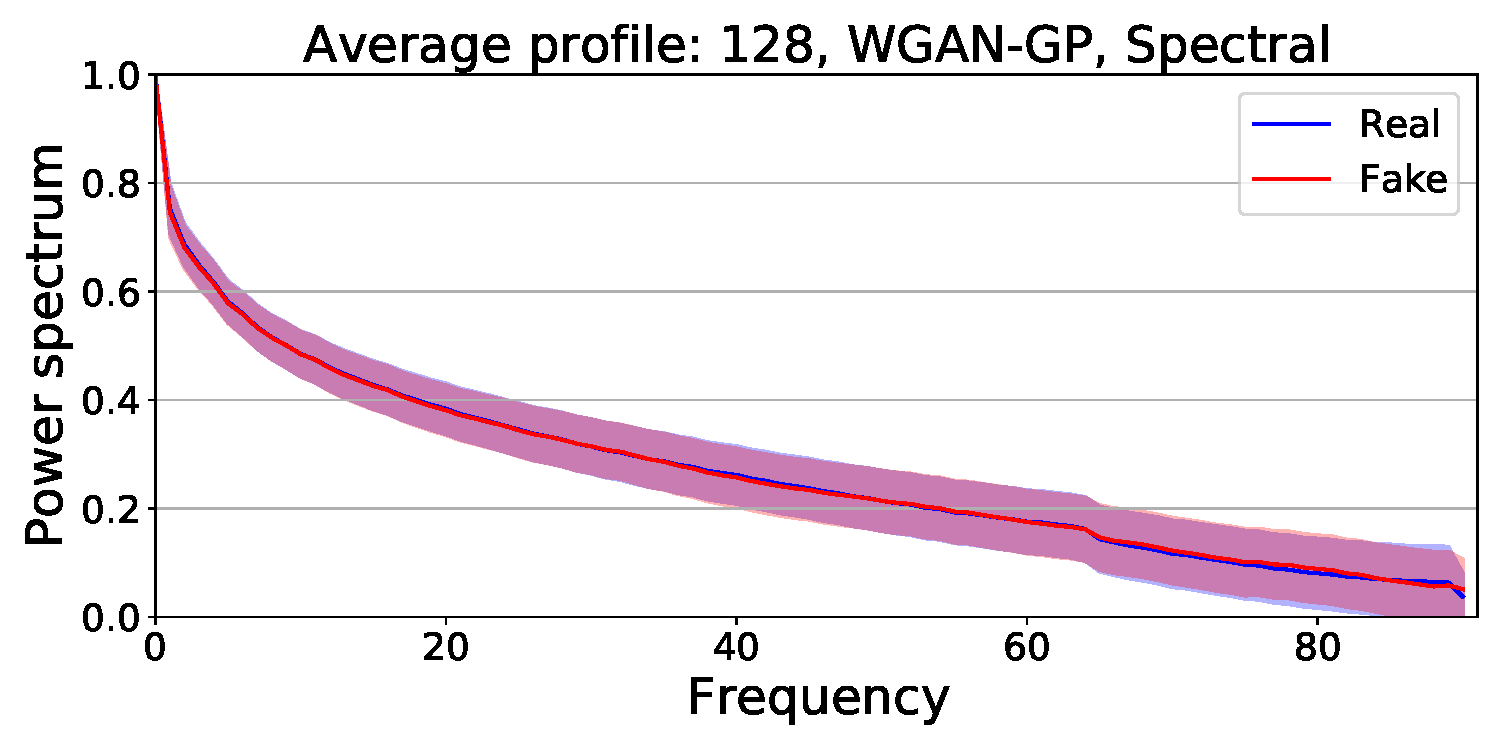
\includegraphics[width=0.49\linewidth]{img/img_2/128_WGAN-GP_Spectral.pdf}\\
        $128\times 128 $ WGAN-GP& WGAN-GP Spectral\\
        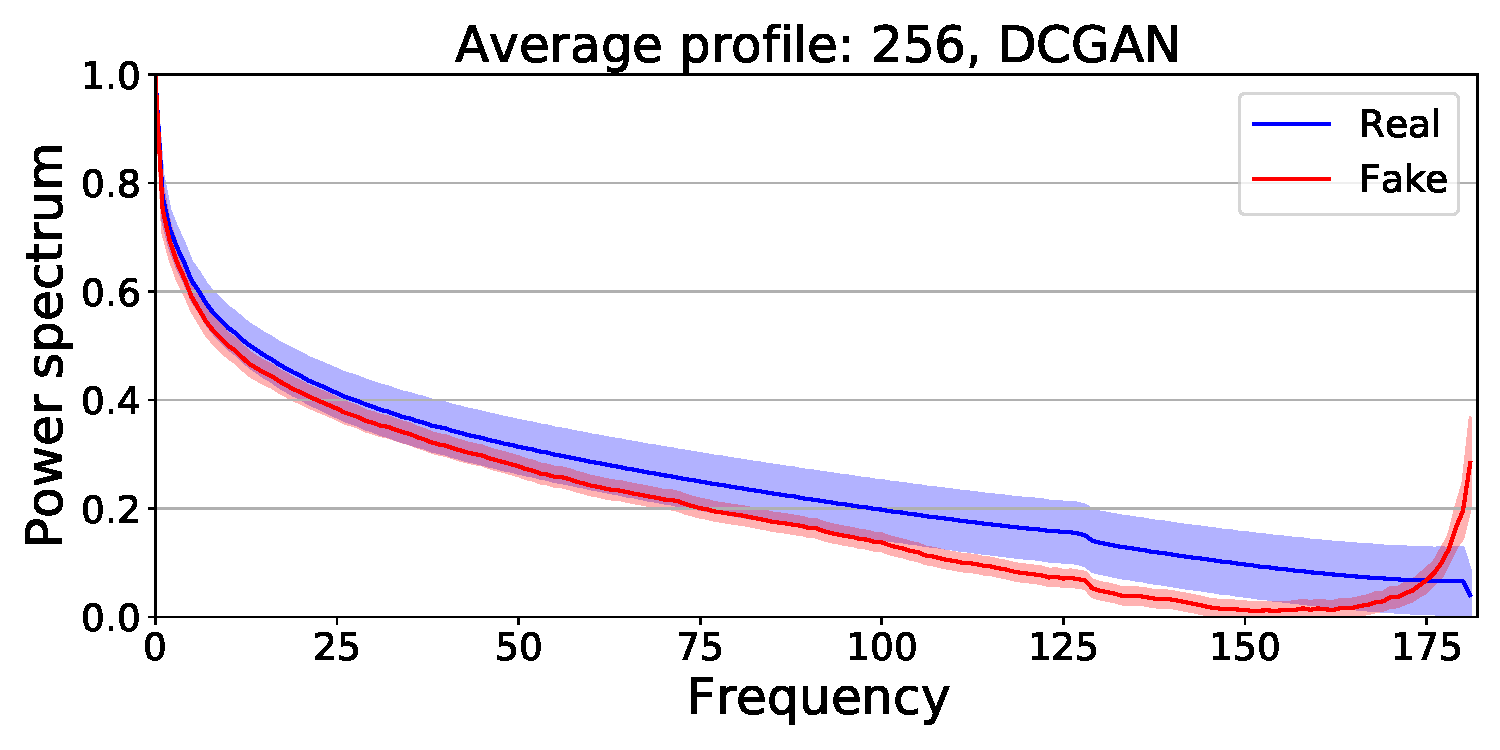
\includegraphics[width=0.49\linewidth]{img/img_2/256_DCGAN.pdf}&
        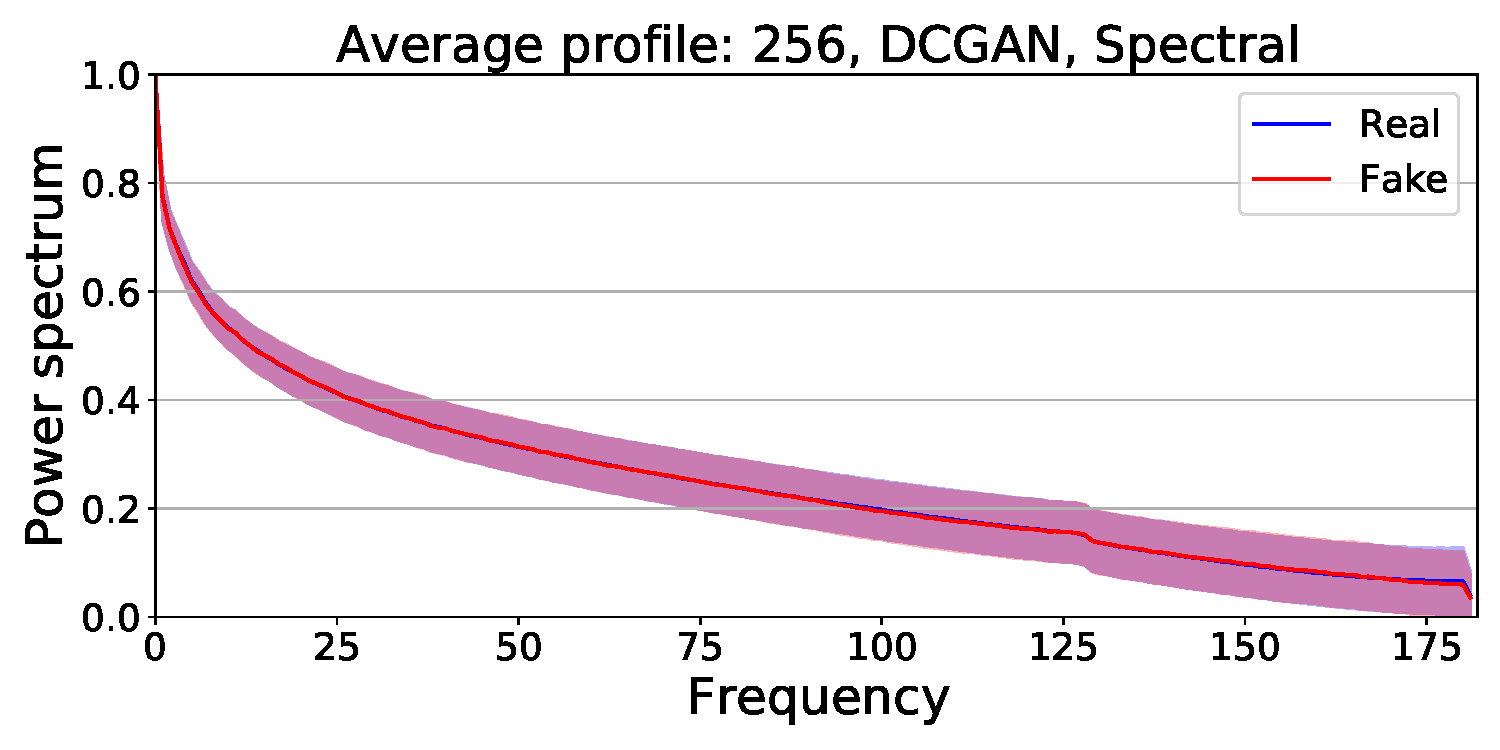
\includegraphics[width=0.49\linewidth]{img/img_2/256_DCGAN_Spectral.pdf}\\
        $256\times 256 $ DCGAN& DCGAN Spectral\\
        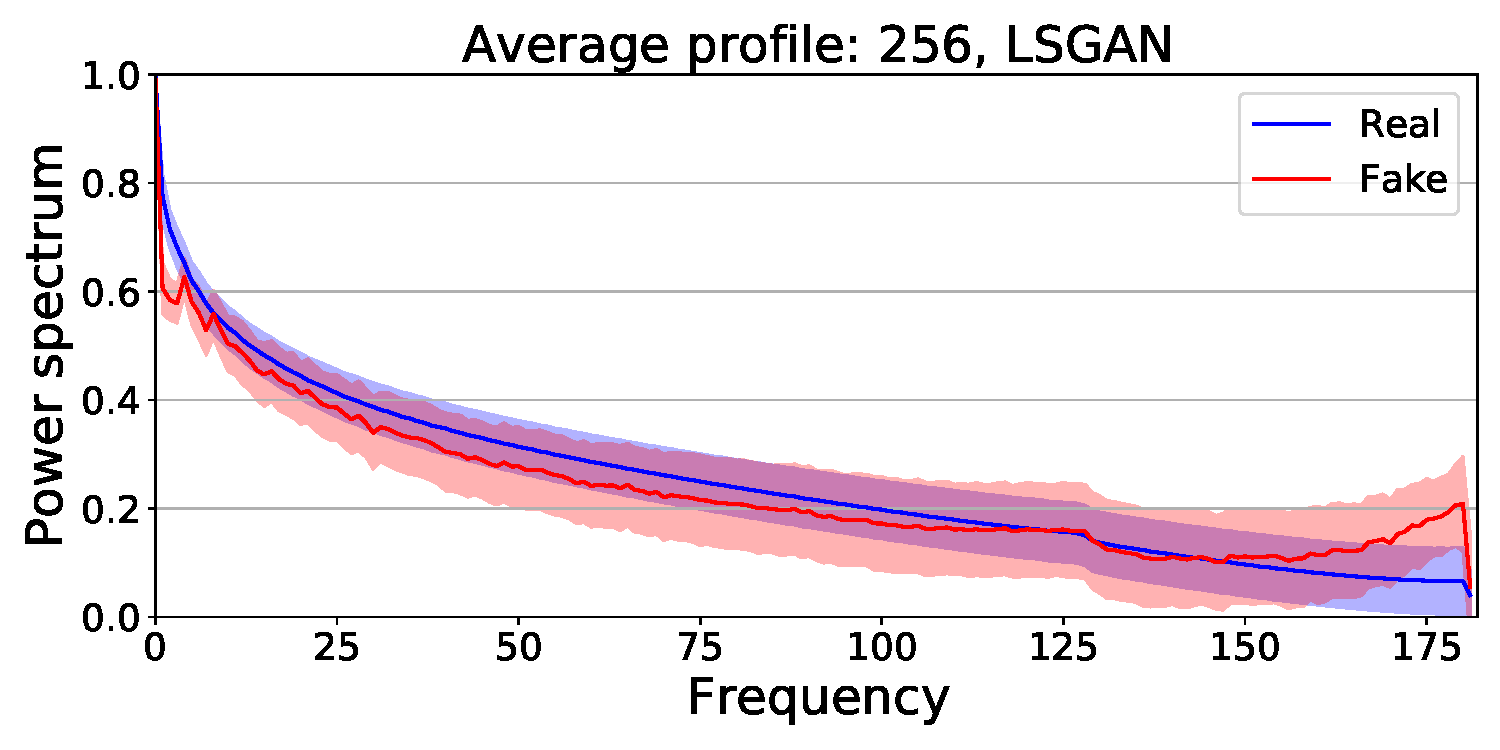
\includegraphics[width=0.49\linewidth]{img/img_2/256_LSGAN.pdf}&
        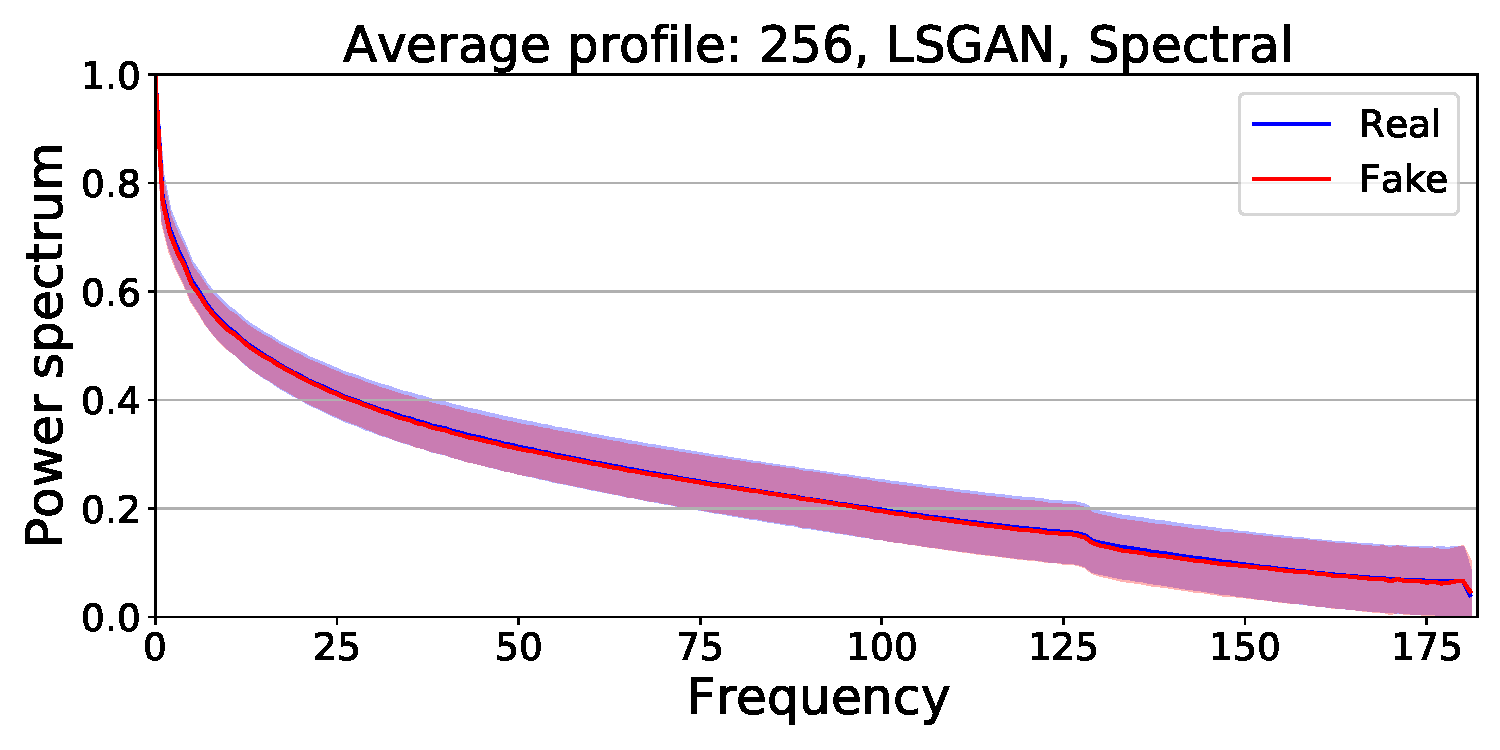
\includegraphics[width=0.49\linewidth]{img/img_2/256_LSGAN_Spectral.pdf}\\
        $256\times 256 $ LSGAN& LSGAN Spectral\\
     
        
     %   \caption{
      %      DCGAN.
      %  }
       % \label{fig:profiles}
    %\end{subfigure}
    %\hfill
    %\begin{subfigure}[t]{.3\textwidth}
    %    \centering
       
    %        LSGAN.
     %   }
     %   \label{fig:profiles}
    %\end{subfigure}
    %\hfill
    %\begin{subfigure}[t]{.3\textwidth}
     % 
        
        
        
      %  \caption{
      %      WGAN.
      %  }
    %    \label{fig:detection}
    %\end{subfigure}
    \end{tabular}
    \caption{
        Experiments with our models trained on FFHQ128 and FFHQ256.
        \emph{Spectral} indicates that $D_F$ was applied. %For the respective higher resolution experiments, see the supplementary material.
         Without the spectral discriminator, the spectral profiles of real and generated images are significantly different in their distribution.
        With the spectral discriminator, the mean and standard deviation of the spectral profiles fit almost perfectly. 
    }
    \label{fig:cloaking2}
    
\end{figure}






\section{Training of the Logistic Regression for the Cloaking Score}
Figure \ref{fig:cdetection} shows the training progress of our regression model used in the cloaking score computation in the section \emph{GAN Evaluation in the Frequency Domain} of the main paper.
Training and testing accuracy are almost identical.
Training accuracy increases progressively to $0.949$ after $100$ epochs, $0.979$ after $1\,000$ epochs, $0.989$ after $10\,000$ epochs, and $0.991$ after $40\,000$ epochs.
We stopped training at this point.
\begin{figure}[t]
        \centering
        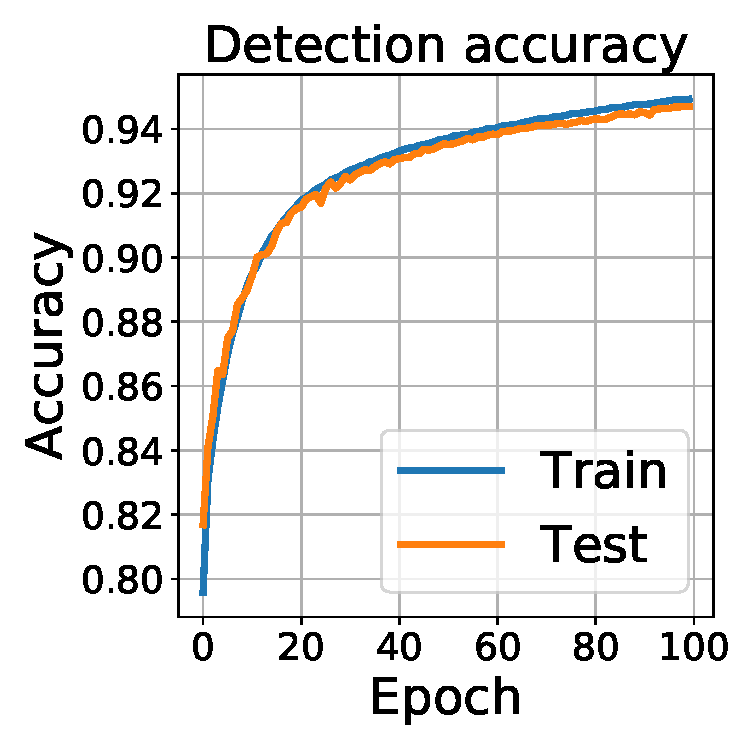
\includegraphics[width=0.6\linewidth]{img/detection_accuracy.pdf}
        \caption{
            Training and test accuracy of a Logistic Regression (LR) trained on $120k$ training images, $60k$ taken from FFHQ and $60k$ generated by StyleGAN2.
            $20k$ images are used for testing. The real and generated images can to a large degree be distinguished using LR.
        }
        \label{fig:cdetection}
    \end{figure}
    \pagebreak
    \pagebreak
\section{Sample images generated from the Proposed Model and the Baselines}
In Figures 6 to 13, we show examples of images generated with DCGAN and LSGAN without and with the proposed spectral discriminator for different resolutions. In all cases, the generated images are visually appealing and diverse.
\iffalse
\begin{figure*}
    
          \centering
        \includegraphics[width=0.6\linewidth]{img/ffhq_average.pdf}
        \includegraphics[width=0.3\linewidth]{img/frequency_hist.pdf}
    \caption{Average spectral profile of FFHQ and the distribution of the last frequency.}
    \label{fig:cloaking}
\end{figure*}
\fi
\iffalse
\begin{table}
    \caption{Detection Scores by Wang et al. (CVPR 20)}
    \label{tab1}
    \centering
    \begin{tabular}{l|l|rr}
        \toprule
       % &&\multicolumn{2}{|c|}{transfer}&\multicolumn{1}{|c|}{}\\
        Size & Model & AP&ACC\\
        \midrule
        
\multicolumn{1}{c|}{\multirow{8}{*}{$64^2$}} 
& DCGAN o& 78.84&67.84 \\
& DCGAN & 89.60&80.81 \\
& DCGAN baseline &78.28&67.09\\
% & DCGAN, Spectral &80.17&68.81\\ 
  & DCGAN, Spectral &77.09&66.35\\ 
 %& DCGAN & 0.85&0.837&0.85&0.84 \\
%& DCGAN baseline & 0.52&0.51&0.73&0.72\\
% & DCGAN, Spectral &0.49 &0.48 &0.57&0.57\\ 
 \cline{2-4}
 & LSGAN &68.61&67.31 \\
 & LSGAN, Spectral &74.29&63.58 \\ \cline{2-4}
 & WGAN & 88.40&78.95\\
 & WGAN, Spectral &  89.11&79.45\\ \cline{2-4}
 & WGAN-GP & 86.07&75.58\\
 & WGAN-GP, Spectral&77.02&65.05\\ \midrule
\multicolumn{1}{c|}{\multirow{8}{*}{$128^2$}} & DCGAN &96.67&81.73\\
 & DCGAN, Spectral & 96.39&80.8\\ \cline{2-4}
 & LSGAN & 96.43&80.53 \\
 & LSGAN, Spectral &96.1&79.7  \\ \cline{2-4}
 & WGAN &96.97&82.93  \\
 & WGAN, Spectral& 96.56&81.20\\ \cline{2-4}
 & WGAN-GP &99.49&95.55  \\ 
 & WGAN-GP, Spectral &86.65&62.44 \\\midrule
\multicolumn{1}{c|}{\multirow{4}{*}{$256^2$}} & DCGAN &99.93& 96.11\\
 & DCGAN, Spectral &99.61&84.79\\ \cline{2-4}
 & LSGAN & 99.53&85.19 \\
 & LSGAN, Spectral &  98.54&72.45\\ \bottomrule
% & WGAN &  \\
% & WGAN, Spectral &  \\ \cline{2-5}
% & WGAN-GP & \\
% & WGAN-GP, Spectral &  \\ \hline

    \end{tabular}
\end{table}
\fi


\iffalse
\begin{figure}[t]
\begin{tabular}{cc}
   % \begin{subfigure}[t]{.3\textwidth}
    %    \centering
        \includegraphics[width=0.49\linewidth]{img/images_DCGAN, Spectral}&
     %   \caption{
      %      DCGAN.
      %  }
       % \label{fig:profiles}
    %\end{subfigure}
    %\hfill
    %\begin{subfigure}[t]{.3\textwidth}
    %    \centering

        \includegraphics[width=0.49\linewidth]{img/images_LSGAN, Spectral.pdf} 
        \\
        DCGAN Spectral & LSGAN Spectral
    %    \caption{
    %        LSGAN.
     %   }
     %   \label{fig:profiles}
    %\end{subfigure}
    %\hfill
    %\begin{subfigure}[t]{.3\textwidth}
     %   \centering

     %   \caption{
      %      DCGAN.
      %  }
       % \label{fig:profiles}
    %\end{subfigure}
    %\hfill
    %\begin{subfigure}[t]{.3\textwidth}
    %    \centering
    %    \caption{
    %        LSGAN.
     %   }
     %   \label{fig:profiles}
    %\end{subfigure}
    %\hfill
    %\begin{subfigure}[t]{.3\textwidth}
     %   \centering

        
      %  \caption{
      %      WGAN.
      %  }
    %    \label{fig:detection}
    %\end{subfigure}
    \end{tabular}
    \caption{
        Images generated by our models trained with DCGAN and LSGAN loss on FFHQ64.
    }
    \label{fig:cloaking3}
\end{figure}
\fi
\iffalse
\begin{figure}[t!]
\begin{tabular}{cc}
   % \begin{subfigure}[t]{.3\textwidth}
    %    \centering
        \includegraphics[width=0.49\linewidth]{img/images_DCGAN.pdf}&
        \includegraphics[width=0.49\linewidth]{img/images_LSGAN.pdf}\\
     %   \caption{
      %      DCGAN.
      %  }
       % \label{fig:profiles}
    %\end{subfigure}
    %\hfill
    %\begin{subfigure}[t]{.3\textwidth}
    %    \centering
        DCGAN  & LSGAN
    %    \caption{
    %        LSGAN.
     %   }
     %   \label{fig:profiles}
    %\end{subfigure}
    %\hfill
    %\begin{subfigure}[t]{.3\textwidth}
     %   \centering

     %   \caption{
      %      DCGAN.
      %  }
       % \label{fig:profiles}
    %\end{subfigure}
    %\hfill
    %\begin{subfigure}[t]{.3\textwidth}
    %    \centering
    %    \caption{
    %        LSGAN.
     %   }
     %   \label{fig:profiles}
    %\end{subfigure}
    %\hfill
    %\begin{subfigure}[t]{.3\textwidth}
     %   \centering

        
      %  \caption{
      %      WGAN.
      %  }
    %    \label{fig:detection}
    %\end{subfigure}
    \end{tabular}
    \caption{
        Images generated by DCGAN and LSGAN.
    }
    \label{fig:cloaking4}
\end{figure}
\fi
\newpage

\begingroup
\setlength\tabcolsep{0pt} % remove whitespace between columns
\renewcommand{\arraystretch}{0}
\centering
\begin{figure}[t]
\begin{tabular}{ccccc}
     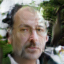
\includegraphics[width=0.18\linewidth]{img/generated_samples/DCGAN64/0088.png} &
     
\includegraphics[width=0.18\linewidth]{img/generated_samples/DCGAN64/0092.png} &
     
\includegraphics[width=0.18\linewidth]{img/generated_samples/DCGAN64/0105.png} &
     
\includegraphics[width=0.18\linewidth]{img/generated_samples/DCGAN64/0109.png} &
     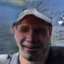
\includegraphics[width=0.18\linewidth]{img/generated_samples/DCGAN64/0134.png} \\
     
\includegraphics[width=0.18\linewidth]{img/generated_samples/DCGAN64/0137.png} &
     
\includegraphics[width=0.18\linewidth]{img/generated_samples/DCGAN64/0144.png} &
     
\includegraphics[width=0.18\linewidth]{img/generated_samples/DCGAN64/0190.png} &
     
\includegraphics[width=0.18\linewidth]{img/generated_samples/DCGAN64/0191.png} &
     
\includegraphics[width=0.18\linewidth]{img/generated_samples/DCGAN64/0199.png} \\
     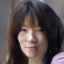
\includegraphics[width=0.18\linewidth]{img/generated_samples/DCGAN64/0205.png} &
     
\includegraphics[width=0.18\linewidth]{img/generated_samples/DCGAN64/0209.png} &
     
\includegraphics[width=0.18\linewidth]{img/generated_samples/DCGAN64/0248.png} &
     
\includegraphics[width=0.18\linewidth]{img/generated_samples/DCGAN64/0274.png} &
     
\includegraphics[width=0.18\linewidth]{img/generated_samples/DCGAN64/0308.png} \\
     
\includegraphics[width=0.18\linewidth]{img/generated_samples/DCGAN64/0418.png} &
     
\includegraphics[width=0.18\linewidth]{img/generated_samples/DCGAN64/0443.png} &
     
\includegraphics[width=0.18\linewidth]{img/generated_samples/DCGAN64/0484.png} &
     
\includegraphics[width=0.18\linewidth]{img/generated_samples/DCGAN64/0620.png} &
     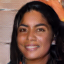
\includegraphics[width=0.18\linewidth]{img/generated_samples/DCGAN64/0991.png}
\end{tabular}
\caption{Generated images, DCGAN, $64^2$.}
\end{figure}
\endgroup

\begingroup
\setlength\tabcolsep{0pt} % remove whitespace between columns
\renewcommand{\arraystretch}{0}
\begin{figure}[t]
\begin{tabular}{ccccc}
     
\includegraphics[width=0.18\linewidth]{img/generated_samples/DCGAN64Spectral/0000.png} &
     
\includegraphics[width=0.18\linewidth]{img/generated_samples/DCGAN64Spectral/0025.png} &
     
\includegraphics[width=0.18\linewidth]{img/generated_samples/DCGAN64Spectral/0027.png} &
     
\includegraphics[width=0.18\linewidth]{img/generated_samples/DCGAN64Spectral/0028.png} &
     
\includegraphics[width=0.18\linewidth]{img/generated_samples/DCGAN64Spectral/0054.png} \\
     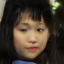
\includegraphics[width=0.18\linewidth]{img/generated_samples/DCGAN64Spectral/0056.png} &
     
\includegraphics[width=0.18\linewidth]{img/generated_samples/DCGAN64Spectral/0105.png} &
     
\includegraphics[width=0.18\linewidth]{img/generated_samples/DCGAN64Spectral/0137.png} &
     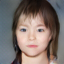
\includegraphics[width=0.18\linewidth]{img/generated_samples/DCGAN64Spectral/0164.png} &
     
\includegraphics[width=0.18\linewidth]{img/generated_samples/DCGAN64Spectral/0180.png} \\
     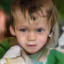
\includegraphics[width=0.18\linewidth]{img/generated_samples/DCGAN64Spectral/0378.png} &
     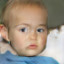
\includegraphics[width=0.18\linewidth]{img/generated_samples/DCGAN64Spectral/0379.png} &
     
\includegraphics[width=0.18\linewidth]{img/generated_samples/DCGAN64Spectral/0385.png} &
     
\includegraphics[width=0.18\linewidth]{img/generated_samples/DCGAN64Spectral/0391.png} &
     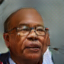
\includegraphics[width=0.18\linewidth]{img/generated_samples/DCGAN64Spectral/0488.png} \\
     
\includegraphics[width=0.18\linewidth]{img/generated_samples/DCGAN64Spectral/0506.png} &
     
\includegraphics[width=0.18\linewidth]{img/generated_samples/DCGAN64Spectral/0508.png} &
     
\includegraphics[width=0.18\linewidth]{img/generated_samples/DCGAN64Spectral/0691.png} &
     
\includegraphics[width=0.18\linewidth]{img/generated_samples/DCGAN64Spectral/0849.png} &
     
\includegraphics[width=0.18\linewidth]{img/generated_samples/DCGAN64Spectral/0935.png}
\end{tabular}
\caption{Generated images, DCGAN, spectral, $64^2$.}
\end{figure}
\endgroup

\begingroup
\setlength\tabcolsep{0pt} % remove whitespace between columns
\renewcommand{\arraystretch}{0}
\centering
\begin{figure}[t]
\begin{tabular}{ccccc}
     
\includegraphics[width=0.18\linewidth]{img/generated_samples/LSGAN64/0000.png} &
     
\includegraphics[width=0.18\linewidth]{img/generated_samples/LSGAN64/0008.png} &
     
\includegraphics[width=0.18\linewidth]{img/generated_samples/LSGAN64/0031.png} &
     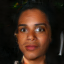
\includegraphics[width=0.18\linewidth]{img/generated_samples/LSGAN64/0066.png} &
     
\includegraphics[width=0.18\linewidth]{img/generated_samples/LSGAN64/0081.png} \\
     
\includegraphics[width=0.18\linewidth]{img/generated_samples/LSGAN64/0095.png} &
     
\includegraphics[width=0.18\linewidth]{img/generated_samples/LSGAN64/0131.png} &
     
\includegraphics[width=0.18\linewidth]{img/generated_samples/LSGAN64/0160.png} &
     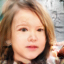
\includegraphics[width=0.18\linewidth]{img/generated_samples/LSGAN64/0235.png} &
     
\includegraphics[width=0.18\linewidth]{img/generated_samples/LSGAN64/0428.png} \\
     
\includegraphics[width=0.18\linewidth]{img/generated_samples/LSGAN64/0431.png} &
     
\includegraphics[width=0.18\linewidth]{img/generated_samples/LSGAN64/0433.png} &
     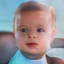
\includegraphics[width=0.18\linewidth]{img/generated_samples/LSGAN64/0446.png} &
     
\includegraphics[width=0.18\linewidth]{img/generated_samples/LSGAN64/0462.png} &
     
\includegraphics[width=0.18\linewidth]{img/generated_samples/LSGAN64/0505.png} \\
     
\includegraphics[width=0.18\linewidth]{img/generated_samples/LSGAN64/0598.png} &
     
\includegraphics[width=0.18\linewidth]{img/generated_samples/LSGAN64/0838.png} &
     
\includegraphics[width=0.18\linewidth]{img/generated_samples/LSGAN64/0859.png} &
     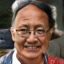
\includegraphics[width=0.18\linewidth]{img/generated_samples/LSGAN64/1016.png} &
     
\includegraphics[width=0.18\linewidth]{img/generated_samples/LSGAN64/1087.png}
\end{tabular}
\caption{Generated images, LSGAN, $64^2$.}
\end{figure}
\endgroup

\begingroup
\setlength\tabcolsep{0pt} % remove whitespace between columns
\renewcommand{\arraystretch}{0}
\begin{figure}[t]
\begin{tabular}{ccccc}
     
\includegraphics[width=0.18\linewidth]{img/generated_samples/LSGAN64Spectral/0001.png} &
     
\includegraphics[width=0.18\linewidth]{img/generated_samples/LSGAN64Spectral/0027.png} &
     
\includegraphics[width=0.18\linewidth]{img/generated_samples/LSGAN64Spectral/0033.png} &
     
\includegraphics[width=0.18\linewidth]{img/generated_samples/LSGAN64Spectral/0052.png} &
     
\includegraphics[width=0.18\linewidth]{img/generated_samples/LSGAN64Spectral/0092.png} \\
     
\includegraphics[width=0.18\linewidth]{img/generated_samples/LSGAN64Spectral/0332.png} &
     
\includegraphics[width=0.18\linewidth]{img/generated_samples/LSGAN64Spectral/0435.png} &
     
\includegraphics[width=0.18\linewidth]{img/generated_samples/LSGAN64Spectral/0505.png} &
     
\includegraphics[width=0.18\linewidth]{img/generated_samples/LSGAN64Spectral/0543.png} &
     
\includegraphics[width=0.18\linewidth]{img/generated_samples/LSGAN64Spectral/0981.png} \\
     
\includegraphics[width=0.18\linewidth]{img/generated_samples/LSGAN64Spectral/1123.png} &
     
\includegraphics[width=0.18\linewidth]{img/generated_samples/LSGAN64Spectral/1415.png} &
     
\includegraphics[width=0.18\linewidth]{img/generated_samples/LSGAN64Spectral/1673.png} &
     
\includegraphics[width=0.18\linewidth]{img/generated_samples/LSGAN64Spectral/1864.png} &
     
\includegraphics[width=0.18\linewidth]{img/generated_samples/LSGAN64Spectral/2075.png} \\
     
\includegraphics[width=0.18\linewidth]{img/generated_samples/LSGAN64Spectral/2085.png} &
     
\includegraphics[width=0.18\linewidth]{img/generated_samples/LSGAN64Spectral/2436.png} &
     
\includegraphics[width=0.18\linewidth]{img/generated_samples/LSGAN64Spectral/2880.png} &
     
\includegraphics[width=0.18\linewidth]{img/generated_samples/LSGAN64Spectral/3093.png} &
     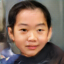
\includegraphics[width=0.18\linewidth]{img/generated_samples/LSGAN64Spectral/3131.png}
\end{tabular}
\caption{Generated images, LSGAN, spectral, $64^2$.}
\end{figure}
\endgroup

\newpage

\begingroup
\setlength\tabcolsep{0pt} % remove whitespace between columns
\renewcommand{\arraystretch}{0}
\begin{figure}[t]
\centering
\begin{tabular}{ccccc}
     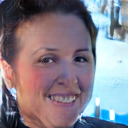
\includegraphics[width=0.32\linewidth]{img/generated_samples/DCGAN128/0000.png} &
     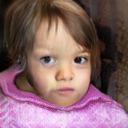
\includegraphics[width=0.32\linewidth]{img/generated_samples/DCGAN128/0001.png} &
     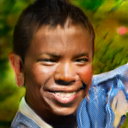
\includegraphics[width=0.32\linewidth]{img/generated_samples/DCGAN128/0014.png} \\
     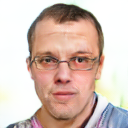
\includegraphics[width=0.32\linewidth]{img/generated_samples/DCGAN128/0076.png} &
     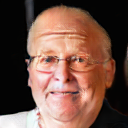
\includegraphics[width=0.32\linewidth]{img/generated_samples/DCGAN128/0080.png} &
     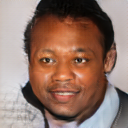
\includegraphics[width=0.32\linewidth]{img/generated_samples/DCGAN128/0085.png} \\
     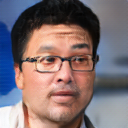
\includegraphics[width=0.32\linewidth]{img/generated_samples/DCGAN128/0294.png} &
     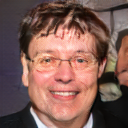
\includegraphics[width=0.32\linewidth]{img/generated_samples/DCGAN128/0387.png} &
     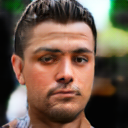
\includegraphics[width=0.32\linewidth]{img/generated_samples/DCGAN128/0398.png}
\end{tabular}
\caption{Generated images, DCGAN, $128^2$.}
\end{figure}
\endgroup

\begingroup
\setlength\tabcolsep{0pt} % remove whitespace between columns
\renewcommand{\arraystretch}{0}
\begin{figure}[t]
\centering
\begin{tabular}{ccccc}
     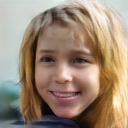
\includegraphics[width=0.32\linewidth]{img/generated_samples/DCGAN128Spectral/0061.png} &
     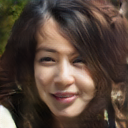
\includegraphics[width=0.32\linewidth]{img/generated_samples/DCGAN128Spectral/0106.png} &
     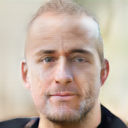
\includegraphics[width=0.32\linewidth]{img/generated_samples/DCGAN128Spectral/0111.png} \\
     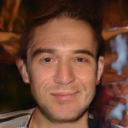
\includegraphics[width=0.32\linewidth]{img/generated_samples/DCGAN128Spectral/0123.png} &
     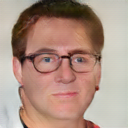
\includegraphics[width=0.32\linewidth]{img/generated_samples/DCGAN128Spectral/0128.png} &
     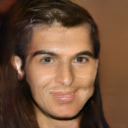
\includegraphics[width=0.32\linewidth]{img/generated_samples/DCGAN128Spectral/0137.png} \\
     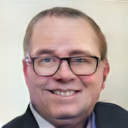
\includegraphics[width=0.32\linewidth]{img/generated_samples/DCGAN128Spectral/0182.png} &
     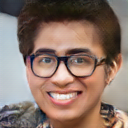
\includegraphics[width=0.32\linewidth]{img/generated_samples/DCGAN128Spectral/0197.png} &
     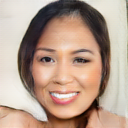
\includegraphics[width=0.32\linewidth]{img/generated_samples/DCGAN128Spectral/0487.png}
\end{tabular}
\caption{Generated images, DCGAN, spectral, $128^2$.}
\end{figure}
\endgroup

\begingroup
\setlength\tabcolsep{0pt} % remove whitespace between columns
\renewcommand{\arraystretch}{0}
\begin{figure}[t]
\centering
\begin{tabular}{ccccc}
     
\includegraphics[width=0.32\linewidth]{img/generated_samples/LSGAN128/0000.png} &
     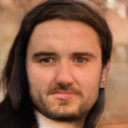
\includegraphics[width=0.32\linewidth]{img/generated_samples/LSGAN128/0012.png} &
     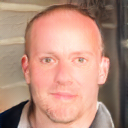
\includegraphics[width=0.32\linewidth]{img/generated_samples/LSGAN128/0135.png} \\
     
\includegraphics[width=0.32\linewidth]{img/generated_samples/LSGAN128/0140.png} &
     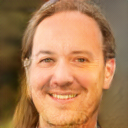
\includegraphics[width=0.32\linewidth]{img/generated_samples/LSGAN128/0284.png} &
     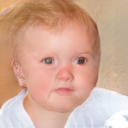
\includegraphics[width=0.32\linewidth]{img/generated_samples/LSGAN128/0311.png} \\
     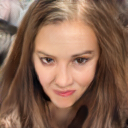
\includegraphics[width=0.32\linewidth]{img/generated_samples/LSGAN128/0599.png} &
     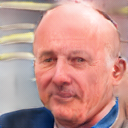
\includegraphics[width=0.32\linewidth]{img/generated_samples/LSGAN128/1270.png} &
     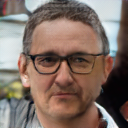
\includegraphics[width=0.32\linewidth]{img/generated_samples/LSGAN128/1273.png}
\end{tabular}
\caption{Generated images, LSGAN, $128^2$.}
\end{figure}
\endgroup

\begingroup
\setlength\tabcolsep{0pt} % remove whitespace between columns
\renewcommand{\arraystretch}{0}
\begin{figure}[t]
\centering
\begin{tabular}{ccccc}
     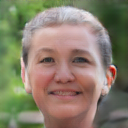
\includegraphics[width=0.32\linewidth]{img/generated_samples/LSGAN128Spectral/0003.png} &
     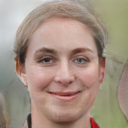
\includegraphics[width=0.32\linewidth]{img/generated_samples/LSGAN128Spectral/0019.png} &
     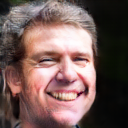
\includegraphics[width=0.32\linewidth]{img/generated_samples/LSGAN128Spectral/0033.png} \\
     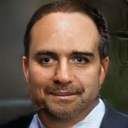
\includegraphics[width=0.32\linewidth]{img/generated_samples/LSGAN128Spectral/0132.png} &
     
\includegraphics[width=0.32\linewidth]{img/generated_samples/LSGAN128Spectral/0385.png} &
     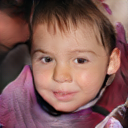
\includegraphics[width=0.32\linewidth]{img/generated_samples/LSGAN128Spectral/0934.png} \\
     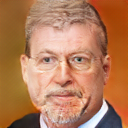
\includegraphics[width=0.32\linewidth]{img/generated_samples/LSGAN128Spectral/1546.png} &
     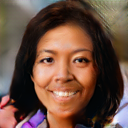
\includegraphics[width=0.32\linewidth]{img/generated_samples/LSGAN128Spectral/2359.png} &
     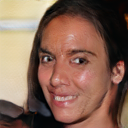
\includegraphics[width=0.32\linewidth]{img/generated_samples/LSGAN128Spectral/2387.png}
\end{tabular}
\caption{Generated images, LSGAN, spectral, $128^2$.}
\end{figure}
\endgroup

\bibliography{manuscrip}
\end{document}


